% Load the document class
\documentclass{univsciauth}

% Other packages
\usepackage{longtable}
\usepackage{chemformula}
\usepackage{longtable}
\usepackage{ltxtable}
\usepackage{tabu}
\usepackage{lipsum}

% siunitx configs
\usepackage[separate-uncertainty, allow-number-unit-breaks]{siunitx}

\DeclareSIUnit{\calorie}{cal}
\DeclareSIUnit\molar{\text{M}}
\DeclareSIUnit\byte{\text{B}}
\DeclareSIUnit\CFU{\text{CFU}}
\DeclareSIUnit\MPN{\text{MPN}}

\usepackage{multirow}

% Document specific configs
\title{
        Molecular techniques for the assessment of Cr (VI) reduction by
        \emph{Bacillus thuringiensis}
}
\shorttitle{Bacterial Cr (VI) reduction}

\author[1]{Deisy L Guerrero-Ceballos*}
\author[1]{Jhonatan Pinta-Melo}
\author[1]{Pablo Fernández-Izquierdo}
\author[2]{Eduardo Ibargüen Mondragon}
\author[1,2]{Edith Mariela Burbano-Rosero}
\authormail{daisymartinez-18@hotmail.com}
\shortauthor{Guerrero-Ceballos et al.}

\Affil{1}{
        Grupo de Investigación en
        Biotecnología Microbiana Universidad de Nariño. 31/10/1993. . Campus
        Universitario Torobajo, Departamento de Biología, Universidad de Nariño,
        Pasto, Colombia.
}
\Affil{2}{
        Grupo de Investigación GIBIMMA. Campus
        Universitario Torobajo, Departamento de Matemáticas, Universidad de
        Nariño, Pasto, Colombia.
}

\funding{
        The VIPRI (Vice-Rectory for Research, Postgraduate Studies and International Affairs), and
        the initiative ``Strengthening regional capacities in research, technological development and innovation
        in the Department of Nariño'' of the CTeI Fund of the General System of Royalties run by the CEIBA
        Foundation in agreement with Gobernación de Nariño.
}

\esmaterial{n.a.}

\doi{10.11144/Javeriana.SC26-2.mtft}

% Start writing your document
\begin{document}
\maketitle
\thispagestyle{firstpage}

\begin{abstract}
Effluent pollution with Cr (VI) is a worldwide
environmental problem. In the Pasto River (southeastern, Colombia),
previous studies reported contamination with this metal at points near
tanneries. To establish the role of \emph{Bacillus thuringiensis} in Cr
(VI) reduction in water from Pasto River, experiments were carried out
with untreated Pasto River water (treatment 1), sterile Pasto
River water inoculated with \emph{B. thuringiensis} (treatment 2), and
unsterilized Pasto River water inoculated with \emph{B. thuringiensis}
(treatment 3). All experiments were conducted in bioreactors with a
controlled temperature of \SI{20}{\celsius} and constant agitation for \SI{156}{h}.
Samples of \SI{20}{mL} were taken every \SI{12}{h} from each treatment to track
Cr (VI) reduction levels and to confirm microorganism identity via
molecular methods involving denaturing gradient gel electrophoresis
(DGGE), restriction enzyme digestion profiles (RFLP), and bioinformatic
analysis. Cr (VI) reduction was higher in treatment 3 (\SI{99.42}{\%}) as
opposed to treatment 2 (\SI{76.12}{\%}) and treatment 1 (\SI{74.46}{\%}). The
molecular identity of \emph{B. thuringiensis} was determined via
sequencing of the 16SrRNA gene, and RFLP assessments in all three
treatments revealed \emph{B. thuringiensis} profiles. Since \emph{B.
thuringiensis} was present in all three treatments trough time, Cr (VI)
reduction can be attributed to this bacterium.

\keywords{Heavy metals; Chromium reduction; Cr reducing
bacteria; DGGE (DeCS).}        
\end{abstract}

\section{Introduction}

Chromium (Cr) is used in several industrial, metallurgical, textile, and
fertilizer activities, resulting in direct and indirect discharges to
main effluents. Often, the amount of chromium discharged exceeds the
maximum concentration established by local or national Environmental
Protection Agencies (EPA) in drinking water (\SI{100}{\micro\gram\per\liter})
{[}1{]}. There
are two states of stability of this metal: trivalent chromium {[}Cr
(III){]} and hexavalent chromium {[}Cr (VI){]}. Although the first state
is not toxic, it has been described that oxidation-reduction processes
can transform it into Cr (VI), a highly toxic, carcinogenic, and
mutagenic state. Cr (VI) has properties of a high degree of corrosion,
solubility in water, and ease of crossing biological membranes, thus
causing alterations in nucleic acids {[}2{]}.

There are different alternatives for the recovery of Cr (VI) from
contaminated effluents, among which bioremediation stands out for its
efficiency and low cost compared to conventional technologies used for
heavy metal removal {[}3{]}. One of the biological systems to be
highlighted is mediated by wild bacteria isolated from contaminated
environments, which have great adaptability at physiological and
metabolic levels, wide functional diversity, and greater efficiency when
implemented in contaminated effluent treatment systems {[}4{]}. In this
sense, Oves \emph{et al.} {[}5{]} evaluated \emph{Pseudomonas
aeruginosa} OSG41 strain tolerance to and reduction capacity of Cr (VI);
the strain was isolated from water contaminated with heavy metals and
the effect of its inoculation was measured on the growth of a chickpea
culture subjected to high concentrations of Cr (VI). The authors
determined that the strain had a high potential for tolerance (up to
\SI{1800}{\milli\gram\per\milli\liter}) and reduction of Cr (VI)
(up to \SI{100}{\%}) depending on physicochemical factors, also reducing the
cytotoxic effect of the metal in chickpea plants.

Consecutively, Hossan \emph{et al.} {[}6{]} studied the efficiency of
reduction and biosorption of Cr (VI) by chromate resistant bacteria
isolated from tannery effluents and established that of the total of
isolated strains, the strain SH-1 characterized as \emph{Klebsiella} sp.
presented Cr (VI) reduction efficiencies of \SI{95.0}{\%} and \SI{63.1}{\%} in the
laboratory and directly in the effluent, respectively. Similarly, Mishra
\emph{et al.} {[}7{]} investigated the Cr (VI) reduction efficiency of
the \emph{Microbacterium paraoxydans} CRB 19 strain, isolated from
chrome-contaminated tannery wastewater from a local common effluent
treatment plant and determined that the bacterium revealed a wide
tolerance to Cr (VI) ($\le \SI{1000}{\milli\gram\per\liter}$) and a reduction
potential that ranges between \SI{39.2}{\%} and \SI{93.5}{\%}.

On the other hand, plant growth promoting rhizobacteria (PGPR) can
increase host plant tolerance to cope up with heavy metal induced
stress, which can improve plant growth. A study carried out by Karthik
\emph{et al.} {[}8{]} isolated a Cr (VI) tolerant PGPR strain and
evaluated its plant growth promoting (PGP) properties under Cr (VI)
stress. The rhizobacterial strain AR6 was isolated from the rhizosphere
of \emph{Phaseolus vulgaris}, this was specifically selected due to its
high Cr (VI) tolerance (\SI{1200}{\micro\gram\per\milli\liter}) and substantial
production of PGP
substances. Inoculation of strain AR6 significantly increased the root
length of test crops in the presence of Cr (VI) and produced a
considerable number of colonizes on the root of versatile dicot and
monocot plants. Moreover, strain AR6 exhibited strong antagonistic
activity against the phytopathogen \emph{Aspergillus niger.} Thus, this
study suggests that metal tolerant and PGP activities of the
rhizobacterial strain AR6 could be exploited for environmental and
agricultural challenges {[}8{]}.

In the department of Nariño, Colombia, there is a high degree of
contamination of effluents by heavy metals, mainly Cr (VI) generated
from leather treatment in tanneries. Chromium concentrations of \SI{59}{mg.L^{-1}}
have been reported in the Pasto River {[}9{]}. A previous study
evaluated the efficiency of the reduction of Cr (VI) by the wild
bacterium \emph{Bacillus thuringiensis} in different treatments using
water from the Pasto River as a substrate {[}10{]}. The results
indicated reduction levels between \SI{74}{\%} and \SI{92}{\%}. In this study,
however, the presence and dynamics of the bacteria during the entire
fermentation process were not determined experimentally with respect to
the bacterial load of the substrate used. Nevertheless, the results are
promising in the context of bioremediation and can be taken as a basis
for implementing decontamination strategies on a large scale.

Molecular techniques and markers aid the characterization of microbial
communities and the detection of microorganisms. One example is
denaturing gradient gel electrophoresis (DGGE). DGGE is a sensitive and
relatively reproducible method central to preliminary studies of
microbial diversity, and its results could be used as a reference for
further investigations where information is complemented in more detail
{[}11{]}. The objective of the present investigation was to determine
the presence of the \emph{B. thuringiensis} bacteria during the Cr (VI)
reduction process in a batch treatment using residual contaminated water
from the Pasto River as a substrate.

\section{Materials and methods}

The microorganisms used in this study were obtained from the
bank of isolates of the Microbial Biotechnology research group at
University of Nariño, which are preserved in \SI{30}{\%} glycerol (GenBank:
MK561610). The isolates were recovered in Luria Bertani (LB)
culture medium at \SI{37}{\celsius} for \SI{24}{h}. An experimental design was
carried out using three treatments with three biological replicates.

The experimental units were bioreactors of \SI{60}{cm} in height and
\SI{11.40}{cm} in diameter. Batch-type fermentation was carried out with a
controlled temperature of \SI{20}{\celsius} and constant agitation at \SI{50}{vvm}
(volume of air per volume of medium per minute). The following treatments were
used:
\begin{itemize}
        \item \textbf{Treatment 1:} Water from the Pasto River without
                sterilization (control without inoculation).
        \item \textbf{Treatment 2:} Sterile water from the Pasto River
                inoculated with \emph{B. thuringiensis}.
        \item \textbf{Treatment 3:} Unsterilized water from the Pasto River
                inoculated with \emph{B. thuringiensis}.
\end{itemize}

The bioreactors were operated for \SI{156}{h}, during which \SI{20}{mL}
samples were taken in sterile \SI{50}{mL} falcon tubes every \SI{12}{h} for total
DNA extraction. To quantify the Cr (VI) reduction of the bacterial
isolates in the water samples, a standard curve was made using the
1,5-diphenylcarbazide method proposed in the 1999 Standards Methods for
the examination of water and wastewater {[}12{]}. Later the samples were
analyzed taking this method into account, namely an aliquot of \SI{5}{mL} of
diluted sample (dilution factor $1/100$) was taken every \SI{12}{h},
H\textsubscript{2}SO\textsubscript{4},
H\textsubscript{3}PO\textsubscript{4}, and 1.5 diphenylcarbazide were
added, homogenized and allowed to stand until the development of the
red-violet color characteristic of complex formation and absorbance at
\SI{543}{nm} was measured. Consecutively, the concentration of Cr (VI) and the
reduction percentage were determined, using the equation of the line
obtained from the standard curve {[}12{]}.

\subsection{Chromosomal DNA extraction}

Total DNA extraction was carried out using the protocol of Burbano and
colleagues. {[}13{]} with modifications in terms of reagent
concentrations, incubation times, and sample volume. First, \SI{20}{mL}
aliquots of water were taken from each treatment at three-time intervals
(\SIlist{0;72;156}{h}). These were centrifuged for \SI{5}{min} at 6461\,$g$.
The supernatant was discarded, and the samples were washed three times
with \SI{500}{\micro\liter} of TE 1X buffer solution, followed by \SI{400}{\micro\liter} of SET buffer
solution {[}\SI{20}{\%} sucrose, \SI{50}{mM} EDTA, and \SI{50}{mM} Tris-HCl, pH
7.6{]}. The tubes were homogenized with a vortex, and \SI{80}{\micro\liter} of lysozyme were
added, followed by incubation at \SI{37}{\celsius} for \SI{1}{h} and \SI{30}{min}
(with shaking every \SI{10}{min}).

Next, \SI{20}{\micro\liter} of \SI{10}{\%} sodium dodecyl sulfate (SDS) solution and
\SI{5}{\micro\liter} of
proteinase K (\SI{20}{mg.mL^{-1}}) were added. The mixture was incubated at
\SI{37}{\celsius}
for \SI{2}{h} with constant shaking. After that, \SI{80}{\micro\liter} of \SI{5}{M} NaCl
and \SI{60}{\micro\liter} of
\SI{10}{\%} hexadecyl trimethyl ammonium bromide (CTAB) were added and
homogenized with a vortex. The mixture was then incubated in a water
bath at \SI{65}{\celsius} for \SI{20}{min} with constant agitation. Then,
$\sim \SI{600}{\micro\liter}$ of phenol-chloroform-isoamyl alcohol (25:24:1)
were added and mixed with a vortex, and the samples were centrifuged at
6461\,$g$ for \SI{10}{min} at room temperature.

The aqueous phase was separated into a new sterile centrifuge tube, and
\SI{1}{\micro\liter} of RNAse (\SI{20}{mg.mL^{-1}}) was added. The mixture was incubated for \SI{1}{h} at
\SI{37}{\celsius}. Additionally, an equal volume of chloroform-isoamyl alcohol
(24:1) was added, a vortex was applied, and the tubes were centrifuged
for \SI{10}{min} at 6461\,$g$ at room temperature. The aqueous phase was
removed and carefully transferred to another new Eppendorf tube. To
achieve DNA precipitation, 0.60 volumes of isopropanol were added to the
tube walls. Once the formation of a precipitate was observed, the tubes
were centrifuged for \SI{10}{min} at 8283\,$g$.

The DNA pellet was washed twice with \SI{200}{\micro\liter} of \SI{70}{\%} ethanol and dried
in an extraction chamber for \SI{15}{min}. Finally, the DNA was resuspended in
\SI{30}{\micro\liter} of ultra-pure water and refrigerated at \SI{-20}{\celsius}. The integrity of
the DNA obtained was verified on \SI{1}{\%} agarose gels (\SI{2}{\micro\liter} of TE 1X, \SI{1}{\micro\liter}
of bromophenol blue, and \SI{2}{\micro\liter} of DNA from each sample) {[}14{]}\emph{.
Lambda HindIII} (Promega; Madison, Wisconsin, USA) was used as the
molecular size marker, and the operating conditions were \SI{70}{V} for \SI{1}{h}
and \SI{30}{min}. The gel was visualized on a Benchtop3UV Transilluminator
photo-documentator at a wavelength of \SI{302}{nm}.

\subsection{PCR amplification of the 16S rRNA gene for DGGE}

The primers 341F-GC + glue GC 5 '(CCTACGGGAGGCAGCAG) 3' {[}15{]} and
907R 5 '(CCGTCAATTCMTTTGAGTTT) 3' {[}15{]} were used for amplification.
PCR reactions were performed at a volume of \SI{50}{\micro\liter}, a final concentration
of \SI{0.40}{\micro M} of primers, a mix of dNTPs at \SI{0.05}{mM}, Taq DNA Polymerase at
\SI{0.025}{U.\micro L^{-1}}, \SI{1}{mM} MgCl\textsubscript{2}, \SI{10}{\micro\liter} of colorless buffer
(Promega; Madison, Wisconsin, USA), and \SI{32.75}{\micro\liter} of sterile ultrapure
water. A DNA template was added for each of the samples at a
concentration of \SI{15}{ng.\micro L^{-1}}. Water was used as a negative control, and
\emph{E. coli} DNA was used as a positive control.

The PCR reaction was performed in a Multigene Labnet thermocycler with
the following thermocycling program: \SI{94}{\celsius} for \SI{10}{min}; 35 cycles of 
\SI{94}{\celsius} for \SI{1}{min}, \SI{54}{\celsius} for \SI{1}{min},
and \SI{72}{celsius} for \SI{2}{min}; and a final
extension of \SI{10}{min} at \SI{72}{\celsius}.

The PCR products were visualized on \SI{1}{\%} agarose gels treated with
ethidium bromide (\SI{5}{\micro g.mL^{-1}}). The gels were run in 1X TAE buffer for \SI{1}{h}
at \SI{70}{V} using \SI{100}{bp} as a molecular size marker (Promega; Madison,
Wisconsin, USA). The gels were visualized on a Benchtop 3UV
Transilluminator photo-documentator at a wavelength of \SI{302}{nm}.

\subsection{DGGE}
PCR products were separated by DGGE. First, a stock solution of
acrylamide - bis acrylamide at a 19: 1 ratio was made from which
denaturant gradients of \SIlist{40;60}{\%} were formed (\autoref{tab:1}).
Polyacrylamide gels were prepared using a TV400-DGGE chamber filling
system (Scie-Plas Ltd.; Cambridge, UK), and then the TAE 1X run buffer
was preheated to \SI{60}{\celsius} for \SI{1}{h}. A pre-run was carried out for
\SI{15}{min} at
\SI{100}{V}. To avoid interference with polyacrylamide residues, gel wells
were washed with run buffer, and then \SI{10}{\micro\liter} of the sample were loaded
from each time interval (\SIlist{0;72;156}{h}) with \SI{5}{\micro\liter} of loading buffer.
\begin{table}[t!]
        \centering
        \caption{
                Standard solutions for denaturing gradient
                formation.
        }\label{tab:1}
        \begin{tabular}{@{}cc@{}}
        \toprule
        \multicolumn{2}{c}{\textbf{Solution of Acrilamida–Bis acrilamida 19:1 (stock)}} \\ \midrule
        \multicolumn{1}{c}{\textbf{Reagents}} & \textbf{Quantitity} \\ \midrule
        Acrilamide & \SI{5.47}{mol} \\
        Bis acrilamide & \SI{0.06}{mol} \\
        Sterile distilled water & Fill to \SI{100}{mL} \\ \midrule
        \multicolumn{2}{c}{\textbf{Solution 0\,\%}} \\ \midrule
        Stock solution & \SI{15}{mL} \\
        Buffer TAE 50X & \SI{2}{mL} \\
        Sterile distilled water & Fill to \SI{100}{mL} \\ \midrule
        \multicolumn{2}{c}{\textbf{Solution 100\,\% (incubation to 37\,°C)}} \\ \midrule
        Stock solution & \SI{15}{mL} \\
        Buffer TAE 50X & \SI{2}{mL} \\
        Deionized Formamide & \SI{40}{mL} \\
        Urea & \SI{6.99}{mol} \\
        Sterile distilled water & Fill to \SI{100}{mL} \\ \midrule
        \multicolumn{2}{c}{\textbf{Denaturing gradient 40\,\%}} \\ \midrule
        Solution \SI{0}{\%} & \SI{9.6}{mL} \\
        Solution \SI{100}{\%} & \SI{6.4}{mL} \\
        TEMED & \SI{12}{\micro L} \\
        Ammonium persulfate \SI{10}{\%} (APS) & \SI{120}{\micro L} \\ \midrule
        \multicolumn{2}{c}{\textbf{Denaturing gradient 60\,\%}} \\ \midrule
        Solution \SI{0}{\%} & \SI{6.4}{mL} \\
        Solution \SI{100}{\%} & \SI{9.6}{mL} \\
        TEMED & \SI{12}{\micro L} \\ 
        Ammonium persulfate \SI{10}{\%} (APS) & \SI{120}{\micro L} \\ \bottomrule
\end{tabular}

\end{table}

An amplicon of the \emph{B. thuringiensis} 16S rRNA gene was used as
comparison standard, and a 100-bp ladder (Promega; Madison, Wisconsin,
USA) was used as the molecular size marker. The running conditions were
\SI{100}{V} and \SI{60}{\celsius} for \SI{5}{h}. After this time, the gel was treated with a
solution of ethidium bromide (\SI{15}{μL} of \SI{1}{\%} ethidium bromide in \SI{100}{mL} of
TAE 1X) for \SI{40}{min} in the dark, washed with sterile distilled water, and
visualized on a Benchtop 3UV Transilluminator photodocumentator at a
wavelength of \SI{302}{nm}.

\subsection{Band selection and purification}
DNA bands without degradation characteristics and with the same position
with respect to the comparison pattern (DNA of \emph{B. thuringiensis})
were selected. To elute the DNA from each of the bands, they were cut
and individually deposited in separate \SI{1.5}{mL} Eppendorf tubes containing
\SI{20}{\micro\liter} of sterile ultrapure water. The tubes were incubated overnight at
\SI{4}{\celsius}. Next, an amplification of the 16SrRNA gene was performed using
\SI{10}{\micro\liter} of the eluate as a template, and the generated amplicons were used
for a second PCR using the same volume of the template (\SI{10}{\micro\liter}).

Additionally, purification of the obtained PCR product was carried out
using an \emph{Illustra GFX PCR DNA} and \emph{Gel Band Purification
Kit} (General Electric; Colombia) according to the manufacturer's
specifications. The product was visualized in a \SI{1}{\%} agarose gel treated
with ethidium bromide at \SI{5}{\micro g.mL^{-1}} with the following running conditions:
\SI{60}{V} for \SI{1}{h}, TAE 1X buffer, and \SI{100}{bp} as the molecular size marker
(Promega; Madison, Wisconsin, USA). The gel was visualized on a Benchtop
3UV Transilluminator photo-documentator at a wavelength of \SI{302}{nm}.

\subsection{Restriction enzyme analysis (RFLP)}

In order to confirm the presence of \emph{B. thuringiensis}
during the reduction process, the amplicons obtained in the second PCR
were digested with three restriction enzymes: \emph{DraI},
\emph{HindIII,} and \emph{HinfI} (Promega; Madison, Wisconsin,
USA). To this end, we worked with a final volume of \SI{20}{\micro\liter}
containing \SI{14.30}{\micro\liter} of sterile deionized water, \SI{2}{\micro\liter} of 10X buffer,
\SI{0.20}{\micro\liter} of BSA (\SI{10}{\micro g.\micro L^{-1}}), \SI{3}{\micro\liter} of the corresponding 16SrRNA gene amplifier
(\SI{1}{\micro g.\micro L^{-1}}), and \SI{0.50}{\micro\liter} of the restriction enzyme (\SI{10}{U.\micro L^{-1}}). Water was
added as a negative control, and \emph{E. coli} DNA was used as a
positive control.

Digestion was carried out for \SI{3}{h} at \SI{37}{\celsius}, and the product
obtained after digestion was visualized in a \SI{1}{\%} agarose gel treated
with ethidium bromide at \SI{5}{μg.mL^{-1}} using the following run conditions:
\SI{60}{V} for \SI{1}{h}, TAE 1X buffer, and \SI{100}{bp} as a molecular size marker
(Promega; Madison, Wisconsin, USA). The result was verified by
in silico tests in the bioinformatics program pDRAW32 version 1.1.130.
The tests were done using sequences of fragments of the \emph{B.
thuringiensis} 16SrRNA gene with a size similar to the study amplicon
(\SI{566}{bp}) from the National Center for Biotechnology Information (NCBI)
database.

\subsection{Bioinformatic analysis of diversity and similarity}

An analysis was performed using the program Photocaptw version
6.0 to calculate the approximate size of the bands located in the same
position with respect to \emph{B. thuringiensis} and those that were
located at different heights. Through this analysis, diversity and
similarity indices (Shannon, Simpson, and maximum likelihood) were
established among the different treatments (Estimates 9.1.0 and Ntsys
2.1). A dendrogram was generated using the program Ntsys version 2.1
(License UH3071IX) according to the coefficient of similarity (maximum
likelihood).

\section{Results}

Chromium reductions of \SI{74.46}{\%}, \SI{76.12}{\%}, and \SI{99.42}{\%} were observed
for treatments 1, 2, and 3, respectively. Notably, these results were
obtained in a previous study. With the modified DNA extraction protocol,
it was possible to obtain samples with quality and concentration greater
than \SI{48}{ng.\micro L^{-1}}. \autoref{fig:1} shows the bands corresponding to the
DNA obtained in each of the treatments with their respective replicates.

\subsection{Amplification of the 16SrRNA gene for DGGE}

\autoref{fig:2} shows the PCR products of the samples from each
treatment (\SI{72}{h} of the Cr (VI) reduction process), which are free of
contamination. This is also reflected in the negative control used in
the process. By comparison with the 100-bp marker, it was established
that the product obtained was approximately \SI{566}{bp}.

\subsubsection{DGGE}

Considering the modifications made in the protocol (mainly in
the amounts of tetramethyl ethylene diamine and ammonium persulfate,
adequate polymerization and runs of the different amplification samples
of the 16S rRNA gene were achieved. \autoref{fig:3} shows the DNA profiles of
each of the treatments analyzed with their respective replicates.

\subsubsection{RFLP}

The \emph{DraI} and \emph{HindIII} enzymes did not generate
fragments of differential sizes, despite \emph{HinfI} generating two
fragments of approximately \SI{650}{bp} and \SI{100}{bp}. Therefore, an
\emph{in-silico} verification was carried out with the program Pdraw 32,
version 1.1.130. The results confirmed that the \emph{DraI} and
\emph{HindIII} do not generate any type of cut in \emph{B.
thuringiensis} sequences (obtained from the base of NCBI data). For this
reason, only \emph{HinfI} was used as reference point (\autoref{fig:4}).

\subsection{Analysis of diversity and similarity}
\begin{figure}[t!]
        \centering
        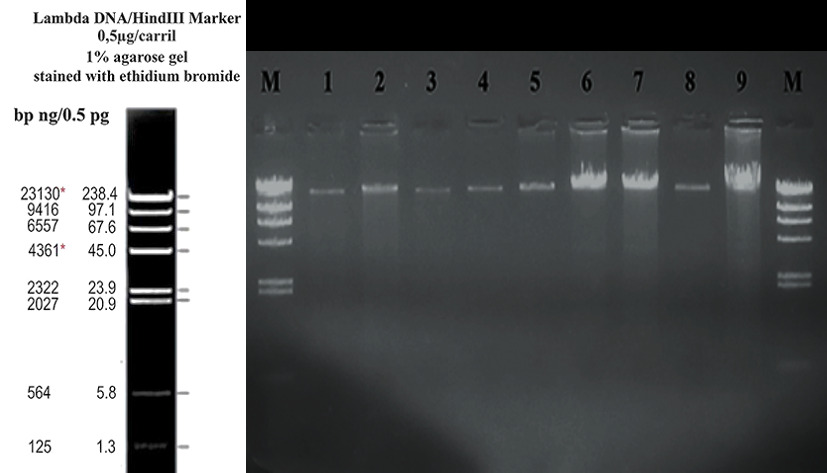
\includegraphics[width=0.8\textwidth]{figures/Figure1.jpg}
        \caption{
                Total DNA extraction (Time 0 of the reduction
                process). The molecular marker (M) Lambda \emph{Hind III}
                (Promega, Madison,Wisconsin,USA) is observed in the first and
                last lane.  First treatment (raw water from Río Pasto) lanes 1
                -3; second treatment (sterile water from Río Pasto inoculated
                with \emph{Bacillus thuringiensis}) lanes 4-6 and third
                treatment (unsterilized water from Río Pasto inoculated with
                \emph{B. thuringiensis}) lanes 7-9. Run conditions: \SI{1}{\%}
                agarose gel, run in 1X TAE buffer at \SI{70}{V} for \SI{1}{h} and
                \SI{30}{min}, treated with \SI{5}{\micro g.mL^{-1}} solution of ethidium bromide and
                photodocumented in the Benchtop3UV Transilluminator kit at a
                wavelength of \SI{302}{nm}.
        }
        \label{fig:1}
\end{figure}
\begin{table}[b!]
        \centering
        \caption{
                Diversity indices of the treatments in three-time intervals:
                first treatment (water from the Río Pasto without sterilizing);
                second treatment (sterile water from Río Pasto + \emph{B.
                thuringiensis}) and third treatment (unsterilized water from
                Río Pasto + \emph{B. thuringiensis).} Tra: treatment and T:
                time.
        }\label{tab:2}
        \resizebox{\textwidth}{!}{
        \begin{tabular}{@{}cccccccccc@{}}
                \toprule
                \textbf{Indices} & \textbf{Tra.1 T0} & \textbf{Tra. 2 T0} & \textbf{Tra.3 T0} & \textbf{Tra.1 T4} & \textbf{Tra.2 T4} & \textbf{Tra.3 T4} & \textbf{Tra.1 T7} & \textbf{Tra.2 T7} & \textbf{Tra.3 T7} \\ \midrule
                \textbf{Taxa} & 3 & 1 & 2 & 3 & 1 & 3 & 3 & 1 & 2 \\
                \textbf{Individuals} & 3 & 1 & 2 & 3 & 1 & 3 & 3 & 1 & 2 \\
                \textbf{Dominance} & 0.3333 & 1 & 0.5 & 0.3333 & 1 & 0.3333 & 0.3333 & 1 & 0.5 \\
                \textbf{Simpson} & 0.6667 & 0 & 0.5 & 0.6667 & 0 & 0.6667 & 0.6667 & 0 & 0.5 \\
                \textbf{Shannon} & 1.099 & 0 & 0.6931 & 1.099 & 0 & 1.099 & 1.099 & 0 & 0.6931 \\ \bottomrule
        \end{tabular}
}

\end{table}

All the bands that were in the gel at the same height of that
corresponding to \emph{B. thuringiensis} had a size of \SI{566}{bp}.
Regarding the Shannon and Simpson indices (\autoref{tab:2}), a low
diversity among samples was evidenced. It should be noted that each
treatment presented the same diversity index at the three times
evaluated, which indicates that the present bacterial populations
probably managed to remain stable in the face of environmental
conditions.

\autoref{fig:5} shows the dendrogram generated by Ntsys version 2.1
(License UH3071IX). The grouping of the different treatments was
established at each time according to the obtained, maximum
likelihood-based coefficients of similarity. The shared similarity
between the treatments was \SI{75}{\%}, indicating the prevalence of \emph{B.
thuringiensis} during the fermentation process. As previously reported,
the dendrogram also reflects similarity levels of \SI{100}{\%} and \SI{76}{\%}
between the three-time intervals in the second and third treatments,
respectively. However, the first treatment presented a similarity of
\SI{46}{\%}.
\begin{figure}[t!]
        \centering
        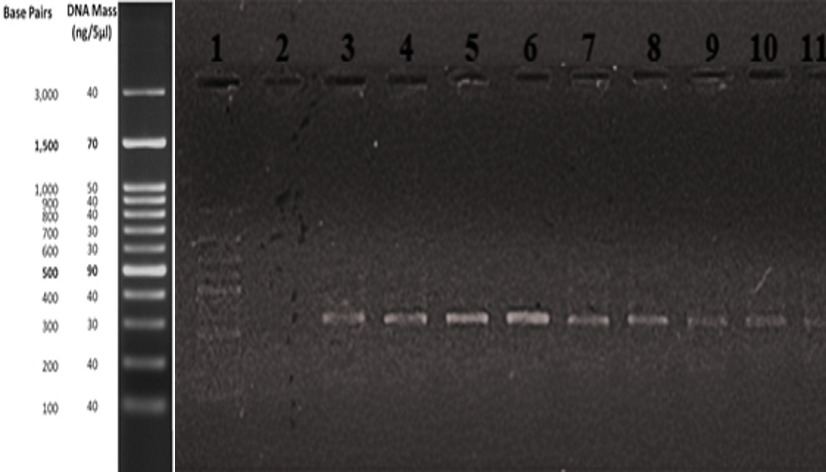
\includegraphics[width=0.8\textwidth]{figures/Figure2.jpg}
        \caption{
                Amplification of the 16SrRNA gene \SI{72}{h} of the
                Cr (VI) reduction process. Lane 2: negative control. First
                treatment (unsterilized water from Río Pasto), lanes 9-11;
                second treatment (sterile water from the Río Pasto inoculated
                with \emph{Bacillus thuringiensis}), lanes 3-5; and third
                treatment (unsterilized water from the Río Pasto inoculated
                with \emph{B. thuringiensis}), lanes 6-8. Size marker is
                observed in the first lane, molecular mass \SI{100}{bp} (Promega,
                Madison, Wisconsin, USA). Run conditions: \SI{1}{\%} agarose gel, run
                in 1X TAE buffer at \SI{70}{V} for \SI{1}{h}, treated with a solution
                of \SI{5}{\micro g.mL^{-1}} of ethidium bromide and photodocumented in the
                Benchtop3UV Transilluminator kit at a wavelength of \SI{302}{nm}.
        }
        \label{fig:2}
\end{figure}
\begin{figure}[t!]
        \centering
        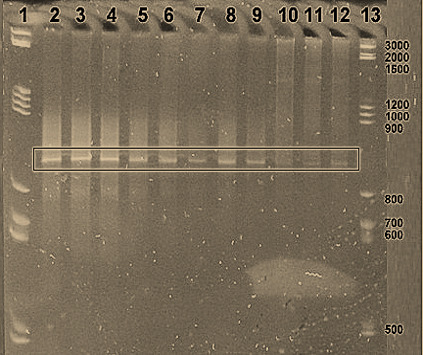
\includegraphics[height=0.6\textwidth]{figures/Figure3.jpg}
        \caption{
                Verification of the denaturing gradient
                electrophoresis process (DGGE) at \SI{156}{h} of the Cr (VI)
                reduction process. Lanes 1 and 13 show the marker of molecular
                size \SI{100}{bp} (Promega, Madison,Wisconsin,USA). First treatment
                (unsterilized water from the Pasto River) lanes 2, 4, and 5;
                second treatment (sterile water from the Río Pasto inoculated
                with \emph{B. thuringiensis}) lanes 10-12; third treatment
                (raw water from Río Pasto inoculated with \emph{B.
                thuringiensis}) lanes 6-8; lanes 3 and 9 DNA of \emph{B.
        thuringiensis}. Run conditions: polyacrylamide gel in \SI{40}{\%} denaturing
        gradient, run in TAE 1X buffer at \SI{100}{V} for \SI{5}{h} at \SI{60}{\celsius},
        treated with a solution of ethidium bromide (\SI{15}{\micro L} of \SI{1}{\%} ethidium
        bromide diluted in \SI{100}{mL} of TAE 1X) and photodocumented on a
        Benchtop3UV Transilluminator equipment at a wavelength of \SI{302}{nm}.
        }
        \label{fig:3}
\end{figure}

\section{Discussion}

The obtained DNA samples showed small traces of contaminants, which are
possibly associated with the fact that the extraction processes in
residual water usually presents interference due to the number of
substances dissolved in the medium, such as organic matter and heavy
metals. According to the physical, chemical, and biological
characteristics of the sample for bacterial DNA extraction, there are
different types of inhibitors that can restrict the adequate recovery of
DNA {[}16,17{]}. However, the analyzed samples presented adequate
characteristics to be processed with different molecular techniques.

It was verified that all the treatments presented higher DNA
concentrations at the first time. In the first treatment, the bands
obtained at \SI{72}{h} and \SI{156}{h} had lower concentrations. This was possibly
caused by the high proportion of Cr (VI) and low concentration of
nutrients from the treatment, which prevented normal growth of the
microorganisms, resulting in population decline {[}18{]}. The obtained
PCR product (\SI{566}{bp}) was that expected for the 16S rRNA gene with the
341F and 907R primers, as found in studies carried out by Faissal
\emph{et al.} {[}19{]}. They reported amplicons between \SIlist{500;550}{bp}
for the 16S rRNA gene with the same primers {[}19{]}.

The bands generated in each of the treatments were positioned at a
similar height with respect to \emph{B. thuringiensis}, which probably
indicates that they are the same bacterial species. However, some
studies exposed the difficulty in separating fragments that differ by 2
or 3 bases due to the high degree of homogeneity in the sequences of
some genes, which occurs with the 16S rRNA gene sequences {[}20-22{]}.
It is possible that a microorganism is represented by several bands. It
is also possible that two different DNA fragments migrate to the same
position in the gel, so that the DGGE profiles are misinterpreted.

It has been determined that errors in the stages prior to the
development of the DGGE technique (DNA extraction and PCR) can introduce
biases in the generated profiles, such as preferential amplifications
and the formation of chimeric molecules and heteroduplex molecules
{[}21, 22{]}. In this sense, it was necessary to complement and verify
the results obtained with cutting with restriction enzymes. In this way,
the restriction enzyme \emph{HinfI} generated two fragments in the study
source samples, similar to those generated in \emph{B. thuringiensis}
(see \autoref{fig:4}). Thus, it could be established that the isolated study
source was present during the fermentation process. For this reason, it
is responsible for the increase in the percentage of reduction of Cr
(VI) in the treatments.
\begin{figure}[t!]
        \centering
        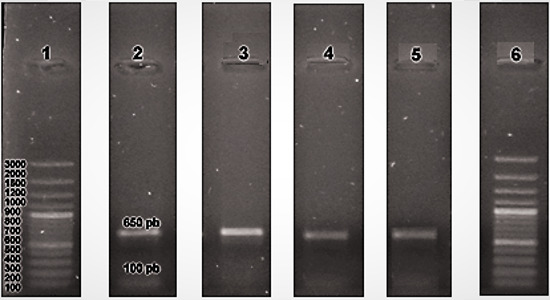
\includegraphics[width=0.8\textwidth]{figures/Figure4.jpg}
        \caption{
                Digestion profile with the endonuclease \emph{HinfI} on
                selected study samples at of the Cr (VI) reduction process.
                Lane 1 shows the marker of molecular size \SI{100}{bp} (Promega,
                Madison,Wisconsin,USA) (M). First treatment (raw water from Río
                Pasto) lanes 4; second treatment (sterile water from Río Pasto
                inoculated with \emph{B. thuringiensis}) lane 2 and third
                treatment (raw water from Río Pasto inoculated with \emph{B.
                thuringiensis}) lane 3; lane 5 \emph{B. thuringiensis} DNA \SI{1}{\%}
                agarose gel, run in 1X TAE buffer at \SI{60}{V} for \SI{1}{h},
                treated with \SI{1}{\%} ethidium bromide solution and photodocumented
                on a Benchtop3UV Transilluminator kit at a wavelength of \SI{302}{nm}.
        }
        \label{fig:4}
\end{figure}

This approach may be a promising alternative for the bioremediation of
contaminated effluents since bacteria isolated from contaminated
environments can present a wide variety of strategies to survive in such
environments {[}23{]}. \emph{Bacillus cereus} was isolated from a coal
mine, and it exhibited different types of stress responses in a medium
supplemented with Cr (VI) {[}23{]}. The results support the process of
chromium reduction through the synthesis of chromoreductases.

Restriction enzymes recognize and cut palindromic sequences, so profiles
generated are specific to a given nucleotide sequence. However, to
ensure the reproducibility of the results, it is necessary to use
several restriction enzymes since there are different critical factors
that can affect and inhibit endonuclease activity. These factors include
DNA purity, temperature, and pH with respect to stability, contaminants
with ($-$) charge, DNA contaminated with other types of DNA, and the
degree of methylation, among others {[}24, 25, 26{]}.

The results obtained in this study are based on two types of molecular
techniques (DGGE and RFLP). The need to use complementary molecular
markers follows the inherent limitations and specific advantages of the
individual approaches (DGGE and RFLP). These methods cannot fully
encompass the complexity of the analysis and study of biological
diversity on their own {[}26{]}. Similar investigations were proposed by
Chai \emph{et al.} {[}27{]}, they evaluated the reducing activity of Cr
(VI) of \emph{Pannonibacter phragmitetus} in bioremediation processes
for contaminated soil and the dynamics of the bacterial population over
time using molecular techniques such as RFLP and real-time PCR. They
concluded that the bacterium presents a potential for application in
bioremediation processes in relation to its population abundance
{[}27{]}.

The Shannon and Simpson indices revealed low diversity between the
samples, which is mainly due to the influence of the high concentration
of Cr (VI) in the medium and the limiting factors. According to Pineda
and Rodríguez {[}3{]}, a low diversity is attributed to a high
concentration of heavy metals that influence the prevalence of bacterial
species capable of tolerating adverse conditions. In addition, factors
such as nutrient limitation, aeration, pH, and temperature can reduce
the number of taxa {[}3{]}. The low level of similarity in the first
treatment may be related to the dynamics of bacterial populations since
the ecosystem in which they were found may be affected by intra- and
interspecific interactions between microorganisms, the presence of
contaminating substances, the amount of available nutrients, oxygen
concentration, pH, and temperature {[}3{]}. These factors cause each
bacterial population to respond in a different way to the stimuli
generated by its microenvironment {[}17, 18{]}.

Treatment 2 presented constant the diversity indices and similarity
coefficients through time. This occurred because a single bacterial
species (\emph{i.e.,} \emph{B. thuringiensis}) was predominant
throughout the Cr (VI) reduction process, thus reflecting the axenic
conditions in which the treatment was maintained. The opposite situation
occurred in the group generated in the other treatments since their
substrate was unsterilized, Pasto River water. Therefore, the bacterial
communities present in the water samples differ significantly depending
on the interaction and medium in which they developed {[}17,18{]}.

Similar studies were proposed by Ma \emph{et al.} {[}28{]}, who
evaluated the reduction of Cr (VI) by a mixed bacterial consortium and
the variation in microbial diversity. In the study done by Ma \emph{et
al.} {[}28{]}, it was possible to determine that this heavy metal
significantly influences the establishment of bacterial communities
{[}28{]}. This was due to the fact that the Shanon and Simpson indices
decreased after the addition of Cr (VI) in the medium. In addition, it
was evident that the genera \emph{Aeromonas},
\emph{Pseudogracilibacillus,} and \emph{Macellibacteroides} predominated
throughout the fermentation process since they expressed specific
functional genes for the elimination of chromium, which allows them to
overcome the environmental conditions and to be selected by the
environment. Similarly, Lin \emph{et al.} performed a characterization
of microbial communities in different wetland substrates to treat Cr
(VI)-contaminated water using molecular techniques such as DGGE and
sequencing. This research used band analysis and diversity indices to
establish that under the stress of Cr (VI), bacterial diversity
decreases significantly, and sensitive bacteria tend to die and become
replaced by bacteria that are tolerant or sensitive to this metal
{[}29{]}.
\begin{figure}[t!]
        \centering
        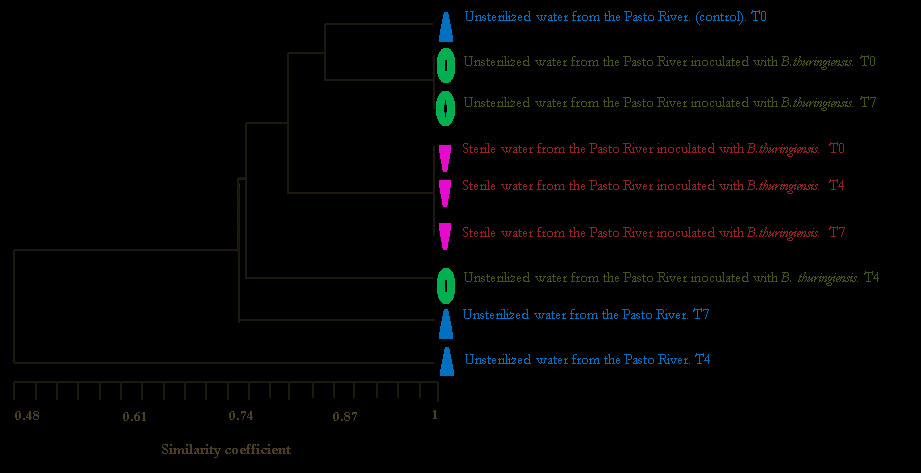
\includegraphics[width=0.8\textwidth]{figures/Figure5.jpg}
        \caption{
                Dendrogram of the treatments analyzed in three stages (maximum
                likelihood coefficient): first treatment (water from the Río
                Pasto without sterilizing); second treatment (sterile water
                from the Río Pasto inoculated with \emph{B. thuringiensis});
                and third treatment (unsterilized water from the Río Pasto
                inoculated with \emph{B.  thuringiensis}). Initial
                concentration of approximately \SI{59}{mg.L^{-1}} of this metal; T0: time
                0, T6: time 6 and T13: time 13 (\SI{0}{h}, \SI{72}{h} and \SI{156}{h}). The
                difference in each of the times is \SI{12}{h} for a total of
                \SI{156}{h} of reduction.
        }
        \label{fig:5}
\end{figure}

On the other hand, Yin \emph{et al.} {[}30{]} evaluated the effect of
cadmium stress on the diversity of a soil microbial community. They
concluded that cadmium pollution significantly changed the structure of
bacterial communities and promoted the growth and development of some
tolerant bacterial species at a low level of cadmium stress of \SI{0.5}{mg.kg^{-1}}.
High levels of cadmium-caused stress significantly inhibited the
growth of \emph{Bacillus thermoamylovorans} and \emph{Bacillus
foraminis}. These preliminary results revealed the response of the soil
microbial community structure to heavy metal pollution and provided a
theoretical reference for early warnings of trends in soil quality
changes.

The different studies cited indicate the importance of characterizing
and determining the dynamics of native bacterial species in environments
contaminated with heavy metals. The ultimate goal is to generate
bioremediation strategies from bacteria that are resistant to these
metals. By means of the molecular markers used, \emph{B. thuringiensis}
was found to be present during the fermentation process. For this
reason, it may be the main responsible for the Cr (VI) reduction process
and is a promising alternative for metal decontamination processes.

\section{Conclusions}

The analyzed treatments presented low diversity indices and high
similarity coefficients (Shannon and Simpson), which is mainly due to
the influence of the high concentration of Cr (VI) in the medium and the
limiting factors such as nutrient limitation, pH and temperature. The
low level of similarity observed in the first treatment may be related
to the dynamics of bacterial populations. This indicates that the
concentration of Cr (VI) can influence the establishment of different
bacterial species. The molecular tools used (DGGE and RFLP) in this
study confirmed that \emph{B. thuringiensis} was present during the Cr
(VI) reduction process in the treatments where it was inoculated, thus
supporting the notion that Cr (VI) reduction is mainly carried out by
this microorganism.

For the technique RFLP, it is advisable to use several restriction
enzymes because different factors can cause the loss of restriction
sites, preventing the generation of the fragments expected by the cuts.
It is important to note that for treatment 2, diversity indices and
similarity coefficient remained constant trough time, reflecting the
axenic conditions in which the treatment was maintained. This approach
may be a promising alternative for the bioremediation of contaminated
effluents since bacteria isolated can present a wide variety of
strategies to survive in such environments.

\section{Acknowledgements}

The authors express their gratitude to the technical personnel of
specialized laboratories of the University of Nariño, to the VIPRI
(Vice-Rectory for Research, Postgraduate Studies and International
Affairs) for the financial resources granted for the execution of the
research, and to the initiative ``Strengthening regional capacities in
research, technological development and innovation in the Department of
Nariño'' of the CTeI Fund of the General System of Royalties run by the
CEIBA Foundation in agreement with Gobernación de Nariño.

\section{Conflict of interest}

The authors declare that they have no affiliations with or involvement
in any organization or entity with any financial interest (such as
honoraria; educational grants; participation in speaker membership,
employment, consultancies, stock ownership, or other equity interest;
and expert testimony or patent arrangements) or non-financial interest
(such as personal or professional relationships, affiliations,
knowledge, or beliefs) in the subject matter or materials discussed in
this manuscript. The authors declare that this work does not entail any
conflict of interest.

\begin{thebibliography}{99}
\bibitem{1} Mädler S, Sun F, Tat C, Sudakova N, Drouin P, Tooley R.
Trace-Level Analysis of Hexavalent Chromium in Lake Sediment Samples
Using Ion Chromatography Tandem Mass Spectrometry, \emph{Journal of
Environmental Protection, 7}: 422--434, 2016.

doi: \href{https://doi.org/10.4236/jep.2016.73037}{10.4236/jep.2016.73037}

\bibitem{2} Xie Y, Holmgren S, Andrews D, Wolfe M. Evaluating the impact of
the US National toxicology program: A case study on hexavalent chromium,
\emph{Environmental health perspectives, 125}: 181--188, 2017.

doi: \href{http://dx.doi.org/10.1289/EHP21}{10.1289/EHP21}

\bibitem{3} Pineda M, Rodríguez A. Metales pesados (Cd, Cr y Hg): su impacto
en el ambiente y posibles estrategias biotecnológicas para su
remediación, \emph{Revista I3+, Investigación, Innovación, Ingeniería},
\emph{2}(2): 82--112, 2015.

doi: \href{https://doi.org/10.24267/23462329.113}{10.24267/23462329.113}

\bibitem{4} Williams P, Botes E, Maleke M, Ojo A, DeFlaun M, Howell J.
Effective bioreduction of hexavalent chromium--contaminated water in
fixed-film bioreactors, \emph{Water SA, 40}(3): 549--554, 2014.

doi: \href{http://dx.doi.org/10.4314/wsa.v40i3.19}{10.4314/wsa.v40i3.19}

\bibitem{5} Oves M., Khan M, Zaidi A. Chromium reducing and plant growth
promoting novel strain Pseudomonas aeruginosa OSG41 enhance chickpea
growth in chromium amended soils, \emph{European journal of soil
biology}, 56: 72--83, 2013.

doi: \href{https://doi.org/10.1016/j.ejsobi.2013.02.002}{10.1016/j.ejsobi.2013.02.002}

\bibitem{6} Hossan S, Hossain S, Islam MR, Kabir MH, Ali S, Islam MS, Mahmud
ZH. Bioremediation of Hexavalent Chromium by Chromium Resistant Bacteria
Reduces Phytotoxicity, \emph{Revista internacional de investigación
ambiental y salud pública}, 17: 6013, 2020.

doi: \href{https://doi.org/10.3390/ijerph17176013}{10.3390/ijerph17176013}

\bibitem{7} Mishra S, Chen S, Saratale G, Saratale R, Ferreira L, Bilal M.,
Bharagava. Reduction of hexavalent chromium by Microbacterium
paraoxydans isolated from tannery wastewater and characterization of its
reduced products, \emph{Journal of Water Process Engineering,} 39:
101748, 2021.

doi: \href{https://doi.org/10.1016/j.jwpe.2020.101748}{10.1016/j.jwpe.2020.101748}

\bibitem{8} Karthik C, Elangovan N, Kumar TS, Govindharaju S, Barathi S,
Oves M, Arulselvi PI. Characterization of multifarious plant growth
promoting traits of rhizobacterial strain AR6 under Chromium (VI)
stress, \emph{Microbiological Research}, 204: 65--71, 2017.

doi: \href{https://doi.org/10.1016/j.micres.2017.07.008}{10.1016/j.micres.2017.07.008}

\bibitem{9} Arango C, Alzate M.
\href{http://www.icesi.edu.co/blogs/gestionintegralindustrial/files/2011/10/SIRAC-Curtiembres.pdf}{\emph{Proyecto gestión ambiental en la industria de curtiembre en Colombia,}}
Pasto, ~\emph{Bogotá DC: Centro Nacional de Producción mas Limpia-Sistema de Referenciación Ambiental (SIRAC) para el Sector Curtiembre en Colombia}. 2004.

\bibitem{10} Guerrero-Ceballos DL, Pinta-Melo J, Fernández-Izquierdo P,
Ibargüen-Mondragón E, Hidalgo-Bonilla SP, Burbano-Rosero EM. Eficiencia
en la reducción de Cromo por una bacteria silvestre en un tratamiento
tipo Batch utilizando como sustrato agua residual del municipio de
Pasto, Colombia,~\emph{Universidad y Salud},~\emph{19}(1): 102--115, 2017.

doi: \href{http://dx.doi.org/10.22267/rus.171901.74}{10.22267/rus.171901.74}

\bibitem{11} Fernández M, Le Borgne S. Electroforesis en gradiente
denaturante. En: Cornejo A, Serrato B, Rendón, Rocha MG,
\emph{Herramientas moleculares aplicadas en ecología: aspectos teóricos
y prácticos}, México, D.F, Primera edición: 14--17, 2014.

\bibitem{12} American Public Health, Association, American Water Works,
Federation, Water Environment. Standards Methods for the examination of
water and wastewater, Chromiun 117A Hexavalente chromiun, In Health AP,
Association AWW, Federation WE, 1999.

\bibitem{13} Burbano-Rosero M, Caetano de Almeida B, Otero-Ramírez I.
\href{https://www.researchgate.net/profile/Edith_Burbano-Rosero/publication/326905291_Manual_de_Biologia_Molecular-Procedimientos_Basicos/links/5b7de35292851c1e12291a22/Manual-de-Biologia-Molecular-Procedimientos-Basicos.pdf}{Manual de Biología Molecular -- Procedimientos Básicos}, \emph{Manual de Biología Molecular -- Procedimientos Básicos}, Pasto, Colombia, 2017: 13--50, 2017.

\bibitem{14} Sambrook J, Fritschi EF, Maniatis T. Molecular cloning: a
laboratorymanual, Cold Spring Harbor Laboratory Press, New York, 1989.

\bibitem{15} Brosius J, Dull TJ, Sleeter D, Noller H. Gene organization and
primary structure of ribosomal RNA operon from \emph{Escherichia coli},
\emph{Journal of molecular biology,} 148: 107--127, 198.

doi: \href{https://doi.org/10.1016/0022-2836(81)90508-8}{10.1016/0022-2836(81)90508-8}

\bibitem{16} Robalino S, Wilson C. 
\href{https://dspace.ups.edu.ec/handle/123456789/14669}{Identificación molecular del complejo Burkholderia cepacia, bacteria productora de antibióticos, mediante PCR en tiempo real}, 
\emph{Disertación Tesis}, Universidad Politécnica
Salesiana, Quito. 2017.

\bibitem{17} Genovese M, Crisafi F, Denaro R, Cappell S, Russo D, Calogero
R, Genovese L. Effective bioremediation strategy for rapid in situ clean
up of anoxic marine sediments in mesocosm oil spill simulation,
\emph{Frontiers in microbiology, 5}(162): 1--14, 2014.

doi: \href{https://doi.org/10.3389/fmicb.2014.00162}{10.3389/fmicb.2014.00162}

\bibitem{18} Barton LL, Northup DE. Microbes at work in nature:
biomineralization and microbial weathering,~\emph{Microbial Ecology},
2011: 299--326, 2011.

\bibitem{19} Faissal , Ouazzani N, Parrado J, Dary M, Manyani H, Morgado B.
Impact of fertilization by natural manure on the microbial quality of
soil: Molecular Approach, \emph{Saudi journal of biological sciences,
24}(6): 1437--144, 2017.

doi: \href{https://doi.org/10.1016/j.sjbs.2017.01.005}{10.1016/j.sjbs.2017.01.005}

\bibitem{20} Shahsavari E, Aburto-Medina A, Khudur LS, Taha M, Ball AS.
Microbial Ecology to Microbial Ecotoxicology. En Cravo-Laureau C, Cagnon
C, Lauga B, Duran R, In~\emph{Microbial Ecotoxicology}, New York:
Springer, 17--38, 2017.

doi: \href{https://doi.org/10.1007/978-3-319-61795-4}{10.1007/978-3-319-61795-4}

\bibitem{21} Fernández M, Le-Borgne S. Electroforesis en gel con gradiente
desnaturalizante, En: Cornejo R, Serrato D, Aguilar B, Munive M,
\emph{Herramientas moleculares aplicadas en ecología: Aspectos teóricos
y prácticos}, SEMARNT INEC UAM-I, 149--170, 2014.

\bibitem{22} Neilson J, Jordan F, Maier R. Analysis of artifacts suggests
DGGE should not be used for quantitative diversity analysis,
\emph{Journal of Microbiological Methods, 92}(2013): 256--263, 2013.

doi: \href{https://doi.org/10.1016/j.mimet.2012.12.021}{10.1016/j.mimet.2012.12.021}

\bibitem{23} Banerjee S, Misra A, Chaudhury S, Dam B. A Bacillus strain TCL
isolated from Jharia coalmine with remarkable stress responses, chromium
reduction capability and bioremediation potential, Journal of hazardous
materials, 367: 215--223, 2019.

doi: \href{https://doi.org/10.1016/j.jhazmat.2018.12.038}{10.1016/j.jhazmat.2018.12.038}

\bibitem{24} Buckhout-White S, Person C, Medintz IL, Goldman ER. Restriction
Enzymes as a Target for DNA-Based Sensing and Structural Rearrangement,
\emph{ACS Omega}, 3(1): 495--502, 2018.

doi: \href{https://doi.org/10.1021/acsomega.7b01333}{10.1021/acsomega.7b01333}

\bibitem{25} Di Felice F, Micheli G, Camilloni G. Restriction enzymes and
their use in molecular biology: An overview, \emph{Journal of
biosciences},~\emph{44}(2): 38, 2019.

doi: \href{https://doi.org/10.1007/s12038-019-9856-8}{10.1007/s12038-019-9856-8}

\bibitem{26} Cruz-Leyva M, Zamudio-Maya M, Corona-Cruz A, González- de la
Cruz J, Rojas-Herrera R.
\href{http://www.scielo.org.mx/scielo.php?pid=S2007-90282015000100008\&script=sci_arttext}{Importancia y estudios de las comunidades microbianas en los recursos y productos pesqueros}, \emph{Ecosistemas y
recursos agropecuarios}, 2(4): 99--115, 2015.

\bibitem{27} Chai L, Yang Z, Shi Y, Liao Q, Min X, Li Q, Liang L. Cr
(VI)-reducing strain and its application to the microbial remediation of
Cr (VI)-contaminated soils, \emph{In Twenty years of research and
development on soil pollution and remediation in China}, 2018: 487--498,
2018.

doi: \href{https://doi.org/10.1007/978-981-10-6029-8_29}{10.1007/978-981-10-6029-8\_29}

\bibitem{28} Ma L, Xu J, Chen N, Li M, Feng C. Microbial reduction fate of
chromium (Cr) in aqueous solution by mixed bacterial consortium,
\emph{Ecotoxicology and environmental safety}, 170: 763--770, 2019.

doi: \href{https://doi.org/10.1016/j.ecoenv.2018.12.041}{10.1016/j.ecoenv.2018.12.041}

\bibitem{29} Lin H, You S, Liu L. Characterization of Microbial Communities,
Identification of Cr(VI) Reducing Bacteria in Constructed Wetland and
Cr(VI) Removal Ability of Bacillus cereus, \emph{Scientific Reports}, 9:
12873, 2019.

doi: \href{https://doi.org/10.1038/s41598-019-49333-4}{10.1038/s41598-019-49333-4}

\bibitem{30} Yin P, Liu X, Liao J, Hu X. Effects of Cadmium Stress on
Microbial Community Diversity in Soil Potted With Sasa Argenteastriatus,
\emph{In IOP Conference Series: Earth and Environmental Science}, 300:
052051, 2019.

doi: \href{https://doi.org/10.1088/1755-1315/300/5/052051}{10.1088/1755-1315/300/5/052051}
        
\end{thebibliography}

\clearpage

\begin{shaded*}
        {\fontsize{11}{10}\selectfont\textbf{\textcolor{myseccolor}{Técnicas moleculares para
        la determinación de la reducción de Cr (VI) por \emph{Bacillus thuringiensis}}}}

        \vspace{3mm}

        {\fontsize{11}{10}\selectfont\textbf{\textcolor{myseccolor}{Resumen:}}}
        La contaminación de efluentes con Cr (VI) es un problema ambiental global. En el rio Pasto
        (sureste de Colombia), estudios previos han reportado contaminación con este metal en
        sitios cercanos a curtiembres. Para establecer el papel de \emph{Bacillus thuringiensis} en la
        reducción de Cr (VI) en el agua del río Pasto, se llevaron a cabo experimentos con aguas
        no tratadas del rio Pasto (tratamiento 1), agua estéril del rio Pasto inoculada con
        \emph{B. thuringiensis} (tratamiento 2) y agua no esterilizada del rio Pasto inoculada con
        \emph{B. thuringiensis} (tratamiento 3). Todos los experimentos se condujeron en biorreactores con
        temperatura controlada de \SI{20}{\celsius} y agitación constante por \SI{156}{h}. Se tomaron muestras de
        \SI{20}{ml} cada 12 horas de cada tratamiento para registrar los niveles de reducción de Cr (VI)
        y confirmar la identidad de los microorganismos por métodos moleculares que
        involucraron electroforesis en gel con gradiente denaturante (DGGE), perfiles de digestión
        de enzimas de restricción (RFLP) y análisis bioinformáticos. La reducción de Cr (VI) fue
        mayor en el tratamiento 3 (\SI{99.42}{\%}) en oposición al tratamiento 2 (\SI{76.12}{\%}) y al
        tratamiento 1 (\SI{74.46}{\%}). La identidad molecular de \emph{B. thuringiensis} se determinó por
        medio de secuenciación del gen 16SrRNA y la determinación de RFLPs en los tres
        tratamientos revelaron los perfiles de \emph{B. thuringiensis}. Dado que \emph{B. thuringiensis} estuvo
        presente en los tres tratamientos a lo largo del tiempo, la reducción de Cr (VI) puede
        atribuirse a esta bacteria.

        {\fontsize{11}{10}\selectfont\textbf{\textcolor{myseccolor}{Palabras Clave:}}} 
        Metales pesados; reducción de cromo; bacterias reductoras de Cr, DGGE
        (DeCS).
\end{shaded*}
%\clearpage
\begin{shaded*}
        {\fontsize{11}{10}\selectfont\textbf{\textcolor{myseccolor}{Técnicas moleculares para avaliar
        redução de Cr (VI) por \emph{Bacillus thuringiensis}}}}

        \vspace{3mm}

        {\fontsize{11}{10}\selectfont\textbf{\textcolor{myseccolor}{Resumo:}}}
        A poluição por efluentes de Cr (VI) é um problema ambiental mundial. Estudos anteriores relataram
        contaminação com este metal em pontos próximos a curtumes no rio Pasto (sudeste da Colômbia). Para
        estabelecer o papel do \emph{Bacillus thuringiensis} na redução de Cr (VI) da água do rio Pasto, realizamos experimentos
        com água do rio Pasto não tratada (tratamento 1), água do rio Pasto esterilizada e inoculada com \emph{B. thuringiensis}
        (tratamento 2) e água do rio Pasto não esterilizada e inoculada com \emph{B. thuringiensis} (tratamento 3). Todos os
        experimentos foram realizados em reatores biológicos com temperatura controlada de \SI{20}{\celsius} e agitação
        constante por \SI{156}{h}. Amostras de \SI{20}{mL} de cada tratamento foram tomadas cada \SI{12}{h} para rastrear a redução
        nos níveis de Cr (VI) e para confirmar a identidade do microrganismos presentes através de métodos
        moleculares como electroforese em gel com gradiente de desnaturação (DGGE), perfis de digestão de
        enzimas de restrição (RFLP), e análises bioinformáticas. A Redução de Cr (VI) foi maior no tratamento 3
        (\SI{99.42}{\%}) do que nos tratamentos 2 (\SI{76.12}{\%}) e 1 (\SI{74.46}{\%}). A identidade molecular de \emph{B. thuringiensis} foi
        determinada por sequenciamento do gene 16SrRNA. Os estudos RFLP dos três tratamentos mostraram perfis
        de \emph{B. thuringiensis}. Uma vez que \emph{B. thuringiensis} esteve presente nos três tratamentos ao longo do tempo, a
        redução de Cr (VI) pode ser atribuída a esta bactéria.

        {\fontsize{11}{10}\selectfont\textbf{\textcolor{myseccolor}{Palavras-chave:}}} 
        Metais pesados; Redução de cromo; Bactérias redutoras de Cr; DGGE (DeCS).
\end{shaded*}
\clearpage
\begin{shaded*}
        {\fontsize{11}{10}\selectfont\textbf{\textcolor{myseccolor}{Deisy Lorena Guerrero Ceballos}}}
        Biologist and Master in Biological Sciences (University of Nariño). Currently a professor at the
        University of Nariño, Colombia. Reach Group on Mathematical Biology and Applied Mathematics
        (GIBIMMA) and Microbial biotechnology.

        ORCID: \href{https://orcid.org/0000-0001-8960-8538}{0000-0001-8960-8538}
\end{shaded*}
\vspace{2mm}
\begin{shaded*}
        {\fontsize{11}{10}\selectfont\textbf{\textcolor{myseccolor}{Jhonatan Pinta Melo}}}
        Biologist and Master in Biological Sciences (University of Nariño). Currently works in the Teaching
        Laboratories of the University of Nariño, Colombia. Researcher of the Research Group in Microbial
        Biotechnology and Mathematical Biology and Applied Mathematics (GIBIMMA).

        ORCID: \href{https://orcid.org/0000-0003-0347-2559}{0000-0003-0347-2559}
\end{shaded*}
\vspace{2mm}
\begin{shaded*}
        {\fontsize{11}{10}\selectfont\textbf{\textcolor{myseccolor}{Edith Mariela Burbano Rosero}}}
        Biologist, master's in Microbiology (Pontificia Universidad Javeriana), Doctor in Science (University
        of São Paulo). Currently research Professor at the University of Nariño, Colombia. Researcher of
        the groups Microbial Biotechnology and Mathematical Biology and Applied Mathematics
        (GIBIMMA) of the University of Nariño. 

        ORCID: \href{https://orcid.org/0000-0002-4021-2660}{0000-0002-4021-2660}
\end{shaded*}
\vspace{2mm}
\begin{shaded*}
        {\fontsize{11}{10}\selectfont\textbf{\textcolor{myseccolor}{Eduardo Ibargüen Mondragon}}}
        Mathematician and Magister in Mathematics (University of Valle), Dr. in Science (National
        Autonomous University of Mexico. Currently Full Professor in University of Nariño (Colombia),
        Reach Group on Mathematical Biology and Applied Mathematic (GIBIMMA).

        ORCID: \href{https://orcid.org/0000-0001-6308-1344}{0000-0001-6308-1344}
\end{shaded*}
\vspace{2mm}
\begin{shaded*}
        {\fontsize{11}{10}\selectfont\textbf{\textcolor{myseccolor}{Pablo Fernández Izquierdo}}}
        Doctor in Biological Sciences, Microbiology and Biotechnology area, Professor of the Department
        of Biology at the University of Nariño, Director of the Microbial Biotechnology research group.

        ORCID: \href{https://orcid.org/0000-0003-0158-8398}{0000-0003-0158-8398}
\end{shaded*}

\end{document}
